\providecommand{\main}{..}
\documentclass[\main/main.tex]{subfiles}

\begin{document}

\lesson{8}{22/10/20}
The idea of generalized brownian motion is to describe the time evolution driven by thermal fluctuations of any microscopic thermodynamic observable $X$ in the framework of FP/Langevin equation. \\

The fact that we deal with finite size systems is crucial in order to fluctuations to take place: we assume that thermal fluctuations are due to independent interactions with a large number of microscopic degrees of freedom. In this way we can apply the CLT and therefore the fluctuations' amplitude scales with system's size like $1/\sqrt{N}$.

The time evolution for a generic thermodynamic observable $X$ driven by fluctuations is given by Langevin equation: 
\begin{align}
    \Tilde{\gamma}\frac{dX}{dt}=\mathcal{F}(X)+\Tilde{\eta}(t)
\end{align}

where we are neglecting the mass term (\textit{overdamped Langevin equation}), $\Tilde{\gamma}$ is a generalized friction coefficient, $\mathcal{F}(X)$ is a thermodynamic force and $\Tilde{\eta}$ is the stochastic noise term:
\begin{equation}
    \mean{\Tilde{\eta}(t)}=0 \quad\mean{\Tilde{\eta}(t) \Tilde{\eta}\left(t^{\prime}\right)}=\Tilde{\Gamma} \delta\left(t-t^{\prime}\right)
\end{equation}

Assuming that noise in uncorrelated at different times implies that our thermodynamic observable is varying on (macroscopic) timescale which are much larger than the microscopic noise correlation time. \\

Using a FP description (in 1d):
\begin{equation}
    \derpars{t}P(X,t)=-\derpars{X}J(X,t)
\end{equation}

where $P$ is the probability distribution and $J$ is a generalized current, defined as:
\begin{equation}
 J(X,t):=v(X)P(X,t)-\underbrace{\frac{\Tilde{\Gamma}}{2\Tilde{\gamma}^2}}_{=D}\derpars{X}P(X,t)
\end{equation}
and the generalized drift velocity is 
\begin{equation}
  v:=\mathcal{F}(X)/\Tilde{\gamma}=\frac{1}{\Tilde{\gamma}}\derpars{X}\mathcal{U}(X) 
\end{equation}


An important role is played by the thermodynamical potential $\mathcal{U}(X)$ which can be defined as a function of the value taken by our thermodynamical observable. We know that the thermodynamical potential is minimum when the observable takes the equilibrium value $X=X^*$ and $\mathcal{U}(X^*)=F(V,T)$ is the \textit{Helmholtz free energy} (assuming we're in the fixed volume/temperature ensemble).

Assuming that my observable $X$ can take different values from equilibrium, this allows us to define the function $\mathcal{U}(X)$. \\

At (local) equilibrium\footnote{Implicitly: whenever $X\neq X^*$ we are globally out of equilibrium but we can still assume a local equilibrium by saying that the probability distribution has a form of a Boltzmann distribution (assuming $k_B=1$): $P(X)=C\exp{-\mathcal{U}(X)/T}$.} we know that $J=0$ and as a consequence we can express the drift velocity as:
\begin{equation}
    v(X)\overset{\Tilde{\Gamma}=2\Tilde{\gamma}T}{=}-\frac{2 T}{\Tilde{\Gamma}}\derpars{X}\mathcal{U}(X)
\end{equation}
which is different from the definition of drift velocity because we have temperature in the equation using the Einstein relation (we can do that because we're at equilibrium)\footnote{We aren't writing equations which are different from the ones we already saw, but the context is different.}. 
Let's now Taylor expand $\mathcal{U}(X)$ around the equilibrium point:
\begin{align}
    \mathcal{U}(X)=F(V,T)+\frac{1}{2}\frac{\partial^2\mathcal{U}}{\partial X^2}\Big\rvert_{X=X^*} (X-X^*)^2+\dots
\end{align}
and if we stop at the second order term this is equivalent to linearize the Langevin equation:
\begin{align}
    \derpars{t}X{=}-\frac{2 T}{\Tilde{\Gamma}}\derpars{X}\mathcal{U}(X)+\frac{\Tilde{\eta}(t)}{\Tilde{\gamma}}\simeq
    \label{qe:lin_la}
\end{align}

the force in general is not a linear function of $X$ but we can linearize (\ref{qe:lin_la}) such that:
\begin{equation}
   \simeq -\frac{2T}{\Tilde{\Gamma}}\chi_{X}^{-1}(X-X^*)+ \frac{\Tilde{\eta}(t)}{\Tilde{\gamma}}
\end{equation}
where $\chi_{X}$ is known as \textbf{thermal (static) susceptibility}:
\begin{align}
   \chi_{{X}}:=\frac{1}{\frac{d^2\mathcal{U}(X)}{dX^2}|_{X=X^*}} 
\end{align}

Neglecting all the other terms in the Taylor expansion we are linearizing the thermodynamic force and the important parameter in this linearization is $\chi_X$. \\

Let's consider the case of a very large susceptibility: $\chi_X>>1$: this means that the second derivative of the potential is very small and therefore we are in a situation like the one represented in Figure \ref{fig:aa}.

\begin{figure}[ht]
    \centering
    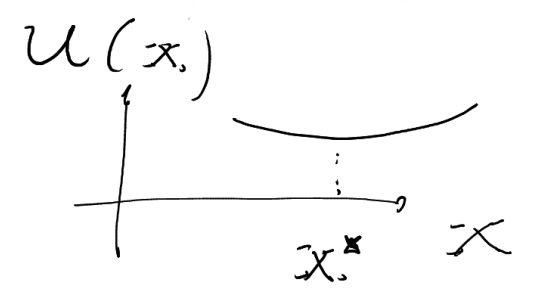
\includegraphics[width=0.5\linewidth]{Lectures/Images/Immagine1.png}
    \caption{Thermodynamic potential $\mathcal{U}$ in the case of $\chi_X>>1$.}
    \label{fig:aa}
\end{figure}

Here the curvature is very small and this means that the restoring force is very small: if we think of this as a spring it would be very loose and so we can push the spring very far but the restoring force would be very small, the system is very susceptible to external perturbations. \\

On the other hand, if $\chi_X<<1$ it means that the potential derivative is very large and so the restoring force is very strong, as we can see from Figure \ref{fig:bb}, where the curvature is very high.

\begin{figure}[ht]
    \centering
    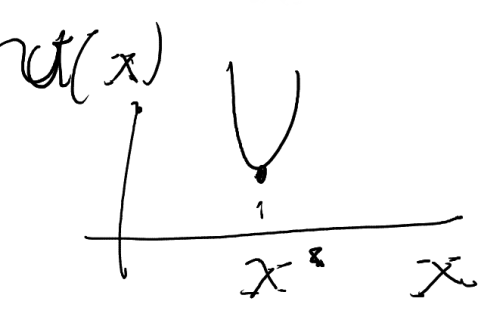
\includegraphics[width=0.5\linewidth]{Lectures/Images/imm2.png}
    \caption{Thermodynamic potential $\mathcal{U}$ in the case of $\chi_X<<1$.}
    \label{fig:bb}
\end{figure}
In this case, even if we moved a little away from equilibrium, the restoring force is already very large and therefore the system is not not really susceptible to external perturbations.

\par\bigskip

\section{Linear response theory introduction}
In this section we will talk about how one uses microscopic dynamics (in particular Hamilton equations) combined with statistical mechanics (Boltzmann-Gibbs ensemble).
\subsection{Microscopic dynamics}
We want to describe N particles (in $d$ dimensions): we will deal with (generalized) positions $q_i(t)$ and momenta $p_i(t)$ with $i=\{1,\dots, N\cdot d\}$.

The Hamilton function is $\mathcal{H}(q_i,p_i)=E$ and we assume in general that energy is conserved; for miscroscopic dynamics we can write down Hamilton equation:
\begin{numcases}{}
\frac{dq_i}{dt}=\frac{\partial\mathcal{H}}{\partial p_i} &\\
\frac{dp_i}{dt}=-\frac{\partial\mathcal{H}}{\partial q_i} &
\end{numcases}

So far we are dealing with \textit{deterministic dynamics} (microscopic reversibility and therefore time reversal invariance) and the point is that forward and backward trajectories are completely determined by initial conditions.

\subsection{Statistical mechanics}
The Boltzmann-Gibbs probability is defined as ($\beta=T^{-1}$):
\begin{align}
    \pi(q_i,p_i)=\frac{1}{Z}\exp{-\beta\mathcal{H}(q_i,p_i)}
\end{align}
where $Z$ is the canonical partition function, $F(V,T)$ the Helmholtz free energy and $\nu$ is the phase space:
\begin{align}
    Z:=\int_{\nu} d\nu \exp{-\beta\mathcal{H}}=\exp{-\beta F(V,T)} \quad d\nu=\frac{1}{N!}\prod_{i=1}^{Nd}(\frac{dq_idp_i}{2\pi\hbar})
\end{align}
Now we have a generic system with its Hamilton function and at what happens at  equilibrium is describable either at microscopic level by Hamilton equation or using statistical mechanics with the partition function. \\

Let's now perturb the Hamiltonian: $\mathcal{H'}:=\mathcal{H}-hX$: the perturbation is $hX$, where $h$ is a perturbation field which is coupled to $X=X(q_i,p_i)$, which is a generic macroscopic thermodynamic observable. 

A way to say that $X$ is coupled to $h$ is to state that $h,X$ are conjugate thermodynamic variables where $h$ is intensive, while $X$ extensive (like $P-V, T-E, \mu-N$). \\

Let's now consider the partition function for the perturbed system:
\begin{equation}
    Z_h=\int_{d\nu}\exp{-\beta\mathcal{H'}}=\exp{-\beta F_{h}}
\end{equation}
where $F_h$ is the \textit{perturbed free energy}.

So far we've perturbed the system but we are still at equilibrium: if we consider the $h$ dependence of $F_h$, this allows me to compute average equilibrium values of my observables as a function of $h$ using 
\begin{equation}
    \derpars{h}F_h=-\mean{X}; \quad \chi_X\overset{(**)}{=}\derpars{h}\mean{X}\overset{(*)}{=}-\derparstwo{h}F_{h}\, (= \frac{1}{\derparstwo{X}\mathcal{U}(X)})
\end{equation}
as a matter of fact we can go from $F_h$ to $\mathcal{U}(X)$ using a \textit{Legendre transform} in order to express the static susceptibility.

Using (*) to express $\chi_X$ we can cast it in this way,  relating it to the variance of $X$:
\begin{equation}
    \chi_X=\beta[\mean{X^2}-\mean{X}^2]
    \label{eq:miaaa}
\end{equation}
In (**) we can see directly that the more the average of $X$ changes when I change $h$, the more the system is susceptible to perturbations but we can already see in (\ref{eq:miaaa}) that, at equilibrium level, this is connected to how much $X$ is fluctuating. 

\paragraph{Example: magnetic susceptibility} In this example $H$ is the magnetic field and $M$ the macroscopic magnetization:
\begin{align}
    \chi=\derpars{H}M=-\derparstwo{H}F=\beta[\mean{M^2}-\mean{M}^2]
\end{align}
where $\mathcal{H'}=\mathcal{H}-HM$.

\section{Linear response theory}

So far we've just discussed equilibrium properties shifted by a perturbing field; now we will consider the response of a system to a \textbf{small} perturbation which is driving the system out-of-equilibrium. 

We will start with an easy case, where the specific time dependent variation of the perturbing field $h$ is described in Figure \ref{fig:pert}, essentially:
\begin{numcases}{h(t)=}
h & $-\infty<t<0$ \\
0 & $t>0$
\end{numcases}

The point is that, at $t=0$, since the perturbation is active since $-\infty$, the system is at equilibrium in the perturbed situation; then $h$ is switched off, so suddenly the system finds itself out-of-equilibrium and therefore what we are interested in is to describe how the system relaxes back to equilibrium for positive times in the absence of a perturbing field.

\begin{figure}[h]
    \centering
    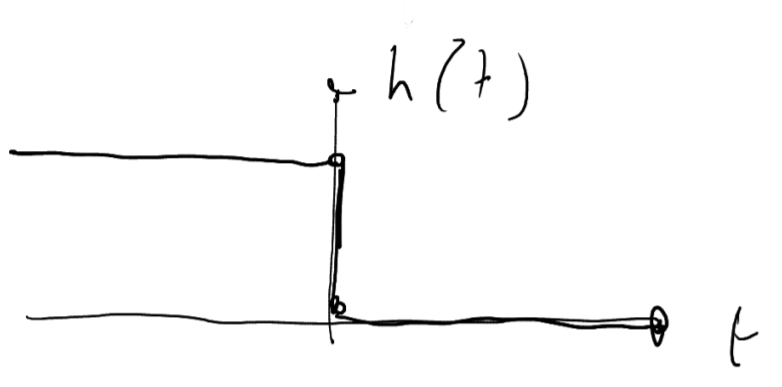
\includegraphics[width=0.5\linewidth]{Lectures/Images/h.png}
    \caption{Time dependent variation of the perturbing filed $h(t)$.}
    \label{fig:pert}
\end{figure}

The relaxation to equilibrium is driven by the thermal bath (by all the interaction with the microscopic degrees of freedom). \\

At $t=0$:
\begin{equation}
    \mean{X}_h \sim \text{equilibrium average for}\,\, \mathcal{H'}
\end{equation}
At $t>0$:
\begin{align}
    X(t) \,\,\text{relaxes to} \,\mean{X}_0
\end{align}
where $\mean{X}_0$ is the new equilibrium value, which is the average for the unperturbed Hamiltonian.

To do that we want to 'mix together' the idea of following the microscopic dynamics given by the Hamilton equation using - at the same time - the Boltzmann-Gibbs ensemble. \\

The crucial point is to follow the behaviour of $X$ as a function of $t$ (which is a non-equilibrium quantity) defining an \textit{out-of-equilibrium average}: not putting the label $_0$ we will consider out-of-equilibrium averages.

The idea is to average over different initial conditions for out-of-equilibrium trajectories: I'm starting in a situation in which I switch off the perturbation and so at $t=0$ the system is out-of-equilibrium; I'm going to follow the dynamics given by the Hamilton equations (how the system relaxes to equilibrium) but I'm considering an ensemble of possible initial conditions for the Hamilton equation and in this sense I'm introducing the idea of considering an out-of-equilibrium average.

To sum up, we are averaging over different relaxation trajectories that starts from different initial conditions:
\begin{equation}
    \mean{X(t)}=\underbrace{\frac{1}{Z_h}\int_{\nu}\exp{-\beta\mathcal{H'}d\nu}}_{I}\underbrace{X(t)}_{II}
    \label{eq:parti}
\end{equation}

The point is, since I know that at $t=0$ what happens is determined by the equilibrium with the perturbed Hamiltonian (at that time $\mean{X}$ e.g. is determined by the equilibrium value with the perturbed Hamiltonian), I'm going to consider the ensemble of possible initial conditions $q_i(0), p_i(0)$ for the Hamilton equations using the B-G ensemble with $\mathcal{H'}$ (using again the fact that the perturbation was ON and constant for all negative times). This is described by part $I$ of equation (\ref{eq:parti}).

In part $II$ we can find the non equilibrium relaxation dynamics implied by the Hamilton equations: formally, when I write this equation
\begin{equation}
    X(t)=X(q_i(t),p_i(t))
\end{equation}
where $q,p$ were obtained by solving the Hamilton equations with initial conditions $q_i(0),p_i(0)$.

What we are doing is considering a given initial condition $q_i(0),p_i(0)$ and then assuming and solving Hamilton equations getting the trajectories $q_i(t),p_i(t)$ and this is defining time evolution of my macroscopic observable $X(t)$. Of course we can't do this in practise and the trick is to average different possible initial conditions, but those are determined by the B-G ensemble of the perturbed Hamiltonian because for all negative times we had the perturbation switched ON at constant value $h$. \\

Let's now assume the small perturbation hypotheses $\beta h<<1$: this means that we can expand (only to the first order) the Boltzmann factor where the perturbation enters
\begin{align}
    \exp{\beta h X}\simeq 1 + \beta h X
    \label{eq:expand}
\end{align}
which allows me to rewrite (\ref{eq:parti}) as:
\begin{align}
    \mean{x(t)}=\frac{\int_{\nu} \exp{-\beta\mathcal{H}(q_i,p_i)}(1+\beta h X(0))d\nu\cdot X(t)\textcolor{blue}{/Z_0}}{\int_{\nu} d\nu \exp{-\beta \mathcal{H}(q_i,p_i)}(1+\beta h X(0))\textcolor{blue}{/Z_0}}=
\end{align}
What we've done is that the Boltzmann factor which is left depends only on the unperturbed Hamiltonian, while in the factor (\ref{eq:expand}) we're considering the initial conditions because is the perturbed one.

the trick now is to divide both the numerator and denominator for the unperturbed partition function $Z_{h=0}=Z_0$ such that now we rewrite N and D as equilibrium averages:
\begin{align}
    \mean{x(t)}=\frac{\mean{(1+\beta h X(0))X(t)}_0}{\mean{1+\beta h X(0)}_0}
\end{align}
\textbf{N.B.}: on the left hand of this equation we have a non-equilibrium average but we manage to express it on the right side using equilibrium averages.

But how are we allowed to conclude that those a re equilibrium averages? Formally $X(t)$ is defined by following the Hamilton equations!

The trick is to change the Boltzmann factor from the perturbed Hamiltonian to the unperturbed one using the small field Taylor expansion. \\

At equilibrium we have time translation invariance (we can think of this as energy conservation) and this means that:
\begin{equation}
    \mean{X(t)}_0=\mean{X}_0
\end{equation}
because it won't depend on time. 

Finally, expanding the denominator as a function of $h$ and rearranging terms:
\begin{equation}
    \boxed{\mean{X(t)}-\mean{X}_0=\beta h [\mean{X(t)X(0)}_0-\mean{X}_0^2]}
    \label{eq:wow}
\end{equation}
This is a first form of a fluctuation-dissipation relations: on the left hand side we find an out-of-equilibrium average and we're describing non-equilibrium relaxation; for infinite time, asymptotically, the left hand side will go to zero (and this is related to dissipation and entropy production).

On the right hand side we see that only equilibrium averages are present and we can see the properties of equilibrium fluctuations encoded in auto-correlation functions.

What this equation is telling us is that both of them decay in the same time and will both go to zero asymptotically. This holds only in the small perturbation limit.

If we have e.g. an exponential decay (and so a characteristic time non equilibrium relaxation or for the decay of the A-C function as a function of time) this equation is telling us that the characteristic time will be the same and so the out-of-equilibrium behaviour is related to the equilibrium behaviour of the A-C function.

\end{document}